Energy Forecasting 

\subsection{Energy forecasting classification}

\subsubsection{Types}
In the context of energy forecasting, the quantities of most interest are price, load and renewables generation.

\subsubsection{Forecasting horizons}
\subsubsection{Size}
- Forecasting horizons

- Refer to section \ref*{metrics} for evaluating metrics

- plots come quelli delle review con i dati di Scopus se é una cosa fattibile
\label{sec:literaturereview}

\begin{figure}[h!]
    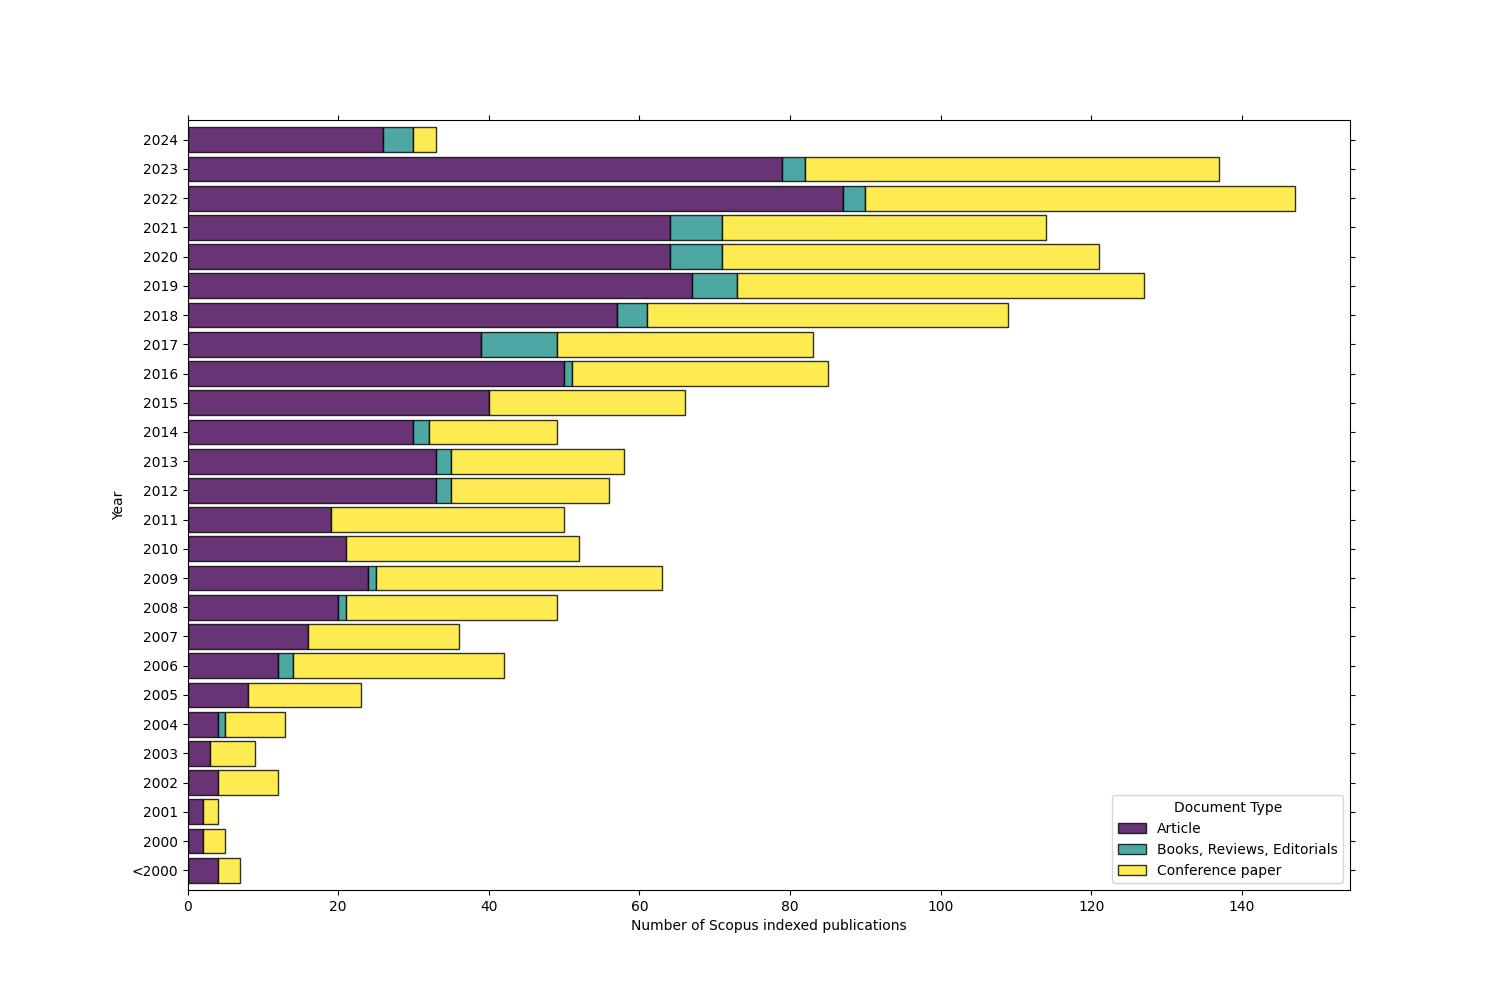
\includegraphics[width=\textwidth]{images/epf_evolution1.jpg}
    \caption{EPF publications \cite{EPF_review}}
    \label{fig:epf_evolution}
  \end{figure}

\begin{figure}[h!]
  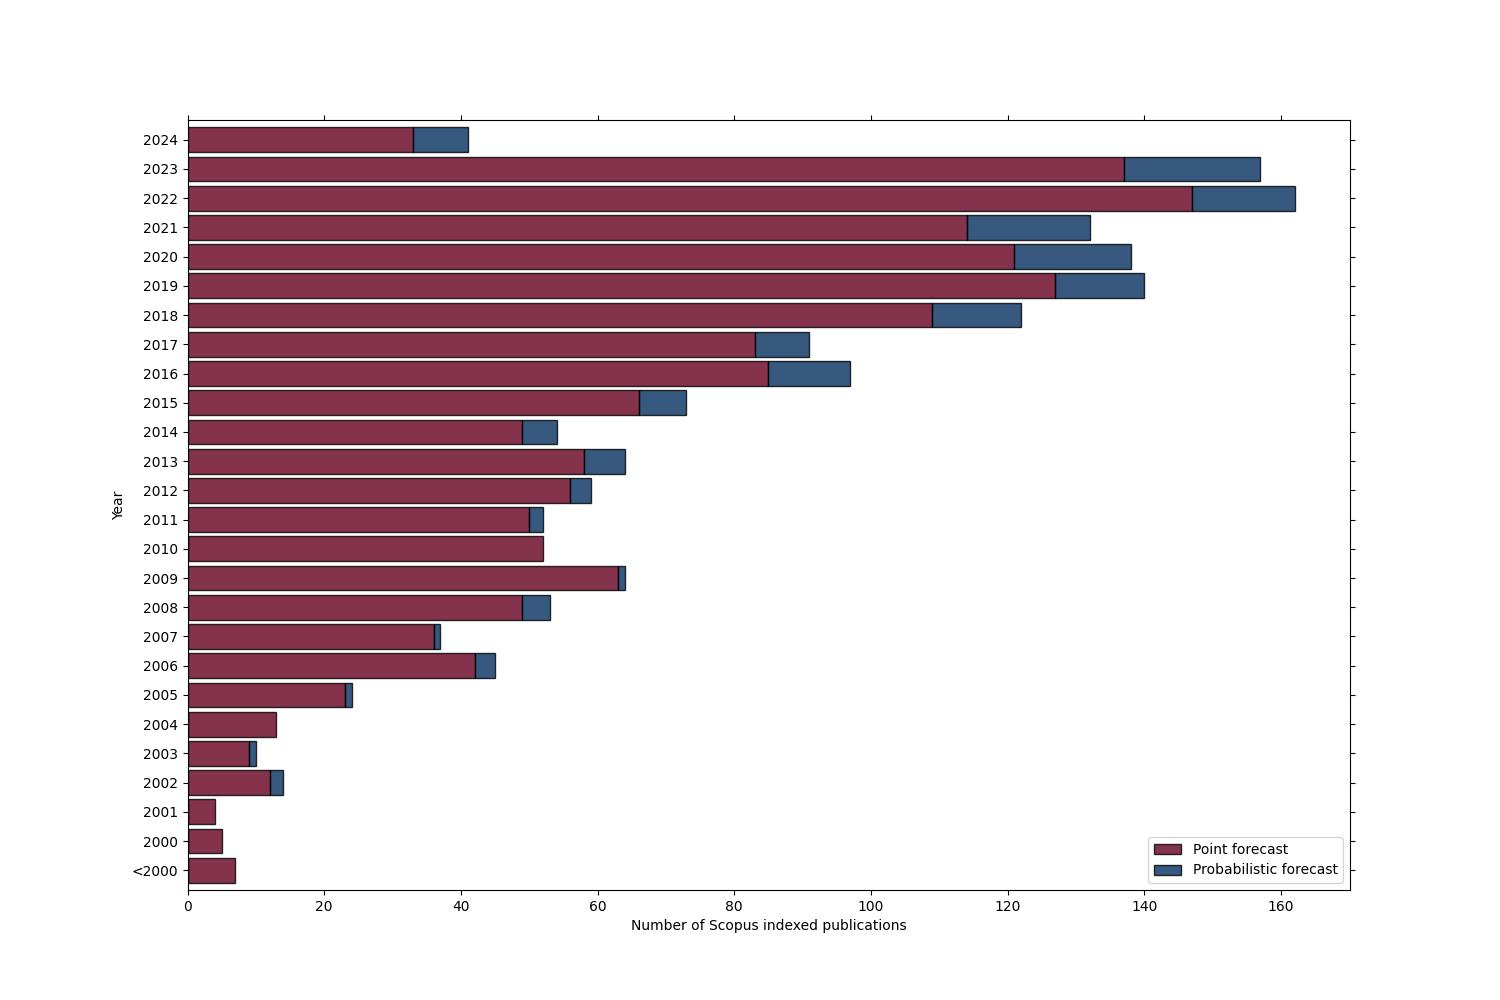
\includegraphics[width=\textwidth]{images/point_vs_prob.jpg}
  \caption{Point vs probabilistic pubblications}
  \label{fig:point_vs_prob}
\end{figure}

\begin{figure}[h!]
  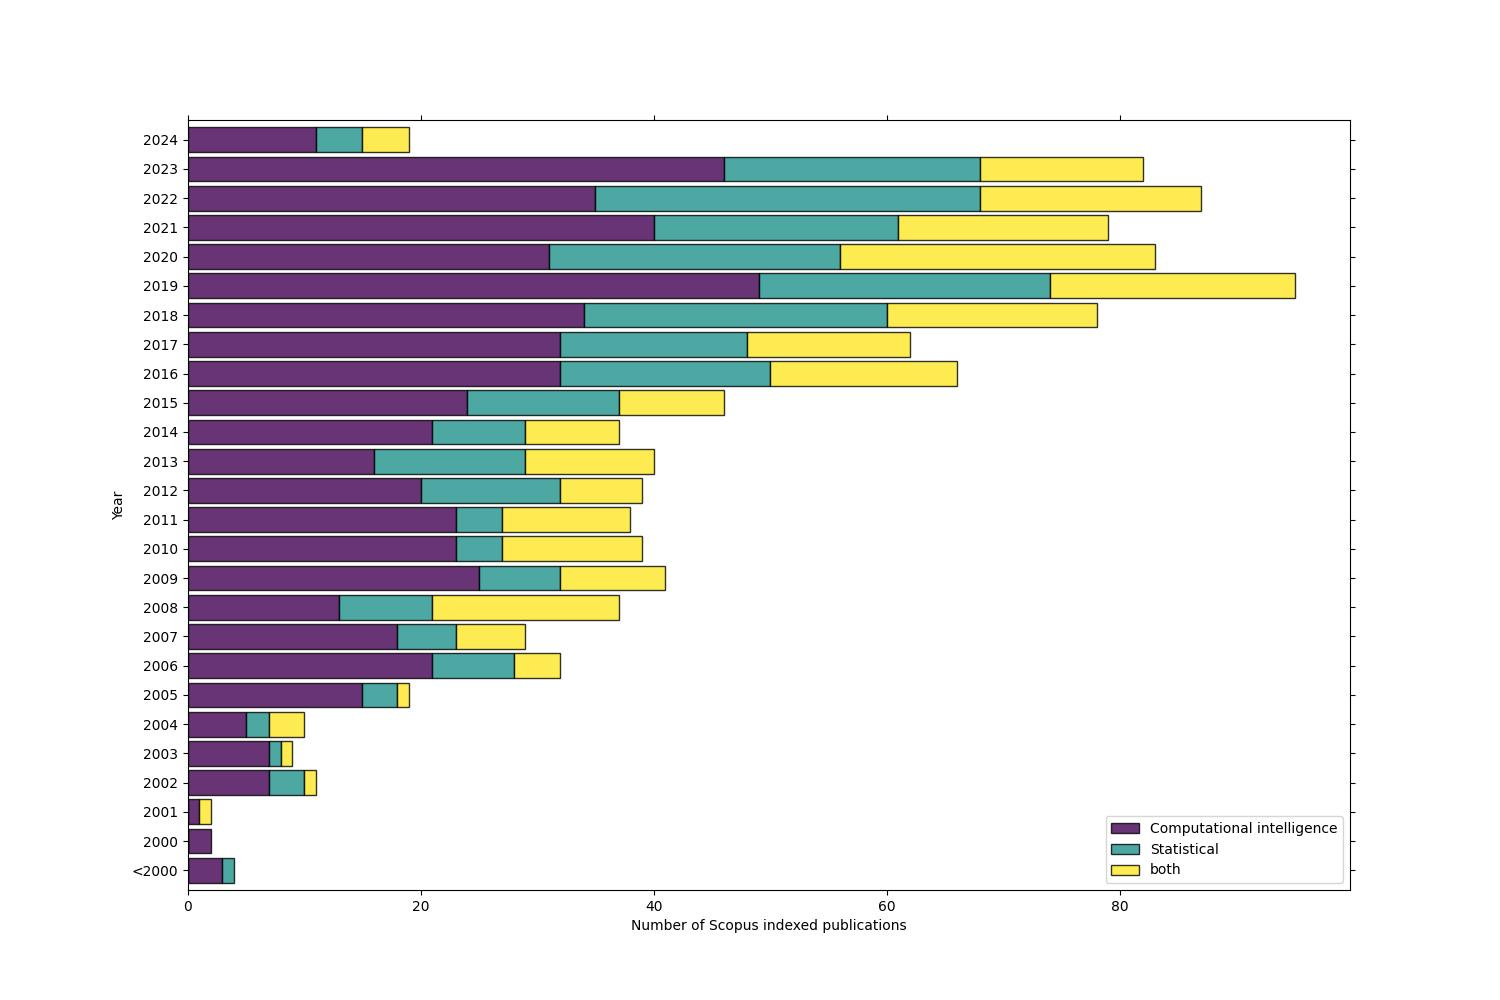
\includegraphics[width=\textwidth]{images/cs_stat_both.jpg}
  \caption{Pubblications by method}
  \label{fig:point_vs_prob}
\end{figure}


\begin{figure}[h!]
  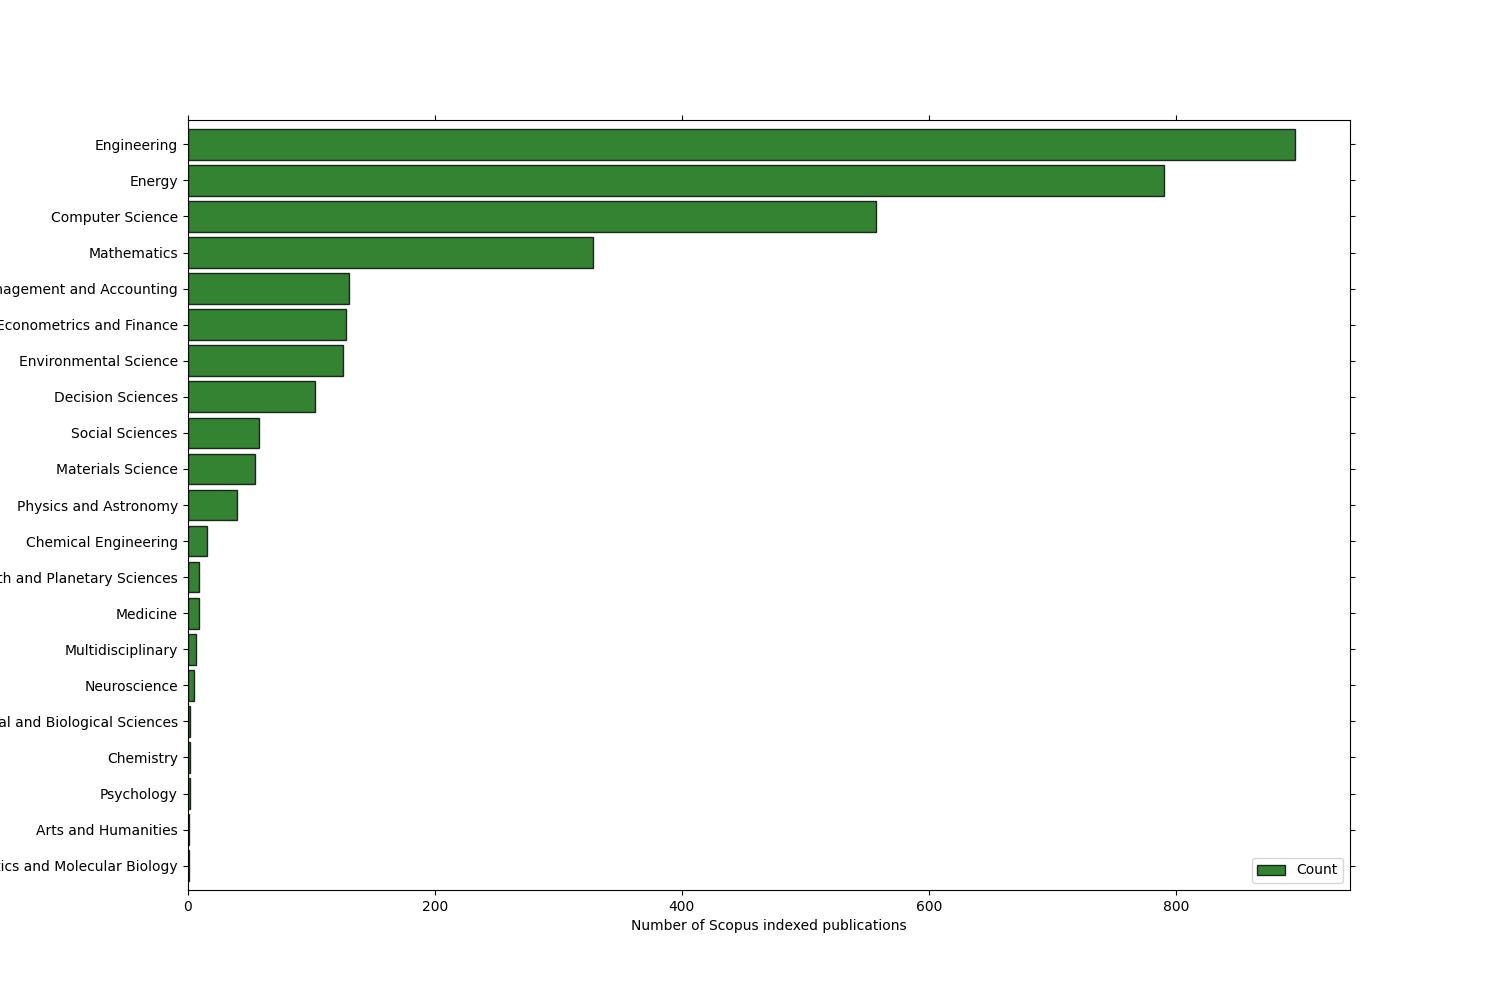
\includegraphics[width=\textwidth]{images/subject_area.jpg}
  \caption{Pubblications by subject area}
  \label{fig:subject_area}
\end{figure}


\begin{figure}[h!]
  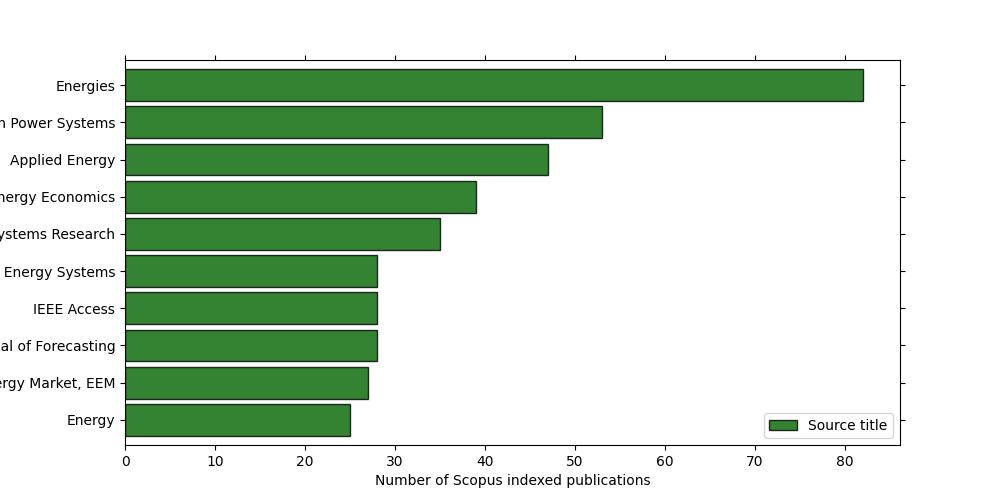
\includegraphics[width=\textwidth]{images/src_title.jpg}
  \caption{Most popolar sources/outlets}
  \label{fig:src_title}
\end{figure}

%INTRO KERNEL METHODS E ENERGY PRICE MODELLING

Kernel methods are a class of algorithms for patter analysis.
With kernel methods we are able to apply linear methods with predictors in a high dimensional space, without having to explicitly evaluate the involved dot products of the features.
In this thesis work I will address the performance of kernel methods in the context of probabilistic forecasting; the area of application will be the electricity market. 
Probabilistic forecasting may be useful to power producers, traders and consumers in order to improve their decision making process and managing risk(VaR). This is because probabilistic forecast enables them to simulate scenarios and carry out stress tests.


%SPIEGO UN PO' I PAPER CHE HO FATTO PASSARE VELOCEMENTE 
Every paper uses different datasets (heterogeneous)
So it is not possible to compare directly results
from one paper to another without implementing the
paper specific algorithms and the applying them to
your dataset.
This is why sections after are destined to analyzing
how these proposed methods so far work and their mathematical
theory details
\\
This problem has been already addressed in \cite{probablistic_electricity_forecast} and \cite{probablistic_electricity_forecast2}. 
These papers surveyed the performance of neural network architectures against simpler approaches like quantile regression and data fitting to Johnson distribution. Their conclusion is that distributional NN perform a little worse than quantile regression but the former has smaller computational cost; that is because the quantile regression is run for every quantile from 0.01 to 0.99.
Nevertheless kernel methods received very little attention in this specific setting.
\\
Kernel methods considered are kernel mean embedding \cite{pmlr}, \cite{Muandet_2017} and kernel herding \cite{supersamples}. Particularly extending the idea of \cite{2022nystrom}, where the Nyström approximation is employed in computing the kernel mean embedding, experiments with the Pivoted Cholesky decomposition will be performed.
\\
In section 2, three papers that lay the basis for this thesis’ work are summarized.
\\
************************
\\
During the past 25 years %because paper of 2014 says 15, so now it is 25
a wide range of new ideas have been proposed for point forecasting and for probabilistic forecasting.
\\
The field benefitted greatly from the increse of computing power, the greater availability of dataset and the interest in data science.
As a consequence, the forecaster's toolbox has grown in size and complexity.
\\
Such variety of methods is characterized by heterogeneity in the fields from which they come from; methods come from statisitics, mathematics, econometrics, electrical engineering and the artificial intelligence communities.
\\
Before delving into the literature review, it is important to make clear that at this point in time there is no superior method. Different solutions may outperform or underperform compared to other techniques depending on the problem settings. Thus, understanding the complexity, strenghts and weaknesses of each method is crucial for fitting the right model to the right setting.
\\
Finally, within this research community, emerged the need of more homogeneity in the choice of the error valuation metrics and in the way of comparing model performances \cite{EPF_review}.
\\
************************
\\
Lately, the idea of combining forecasts has gained popularity in the forecasting communit \cite{forecasting_big}; in the literature, combined forecasts are called ensemble \cite{gneiting_weather_ensemble}.
Experimental results have shown ensemble methods to outperform their component forecasts.
\\
Note that the more the errors of the combined models are not correlated the more we can benefit from ensembles.
\\
It is also worth noting that older and simpler methods are still valuable(in combination with other models or on their own); these being less subject to overfitting than complex models.
